\section{Preliminaries}
This section presents the employed system model, notation, and the considered control problem.

\subsection{System model}\label{sec:sys_model}
Consider a non-deterministic discrete \ac{LTI} system $\mathcal{S}$ whose dynamics is described in the so-called \textit{innovation} form by
\begin{subequations}\label{eqn:SS_innovation}
\begin{empheq}[left=\mathcal{S}_\mathcal{I}\empheqlbrace]{align}
    x_{k+1} &= Ax_k + Bu_k + Ke_k,\label{eqn:SSi_x}\\
	y_k &= Cx_k + Du_k + e_k \label{eqn:SSi_y},
  \end{empheq}
\end{subequations}
in which the subscript $k\in\mathbb{Z}$ denotes the discrete time index, ${x_k\in\mathbb{R}^n}$, ${u_k\in\mathbb{R}^r}$, ${y_k\in\mathbb{R}^l}$, ${e_k\in\mathbb{R}^l}$ respectively represent states, inputs, outputs, and zero-mean white innovation noise with variance $R_\mathrm{e} \succ 0$, and $\{A,B,C,D,K\}$ are system matrices of compatible dimensions. Henceforth it is assumed that the input and output sequences of $\mathcal{S}$ are (jointly) quasi-stationary second-order ergodic stochastic processes. This ensures that limits of time averages involving these sequences exist and that sample correlations approach a finite true correlation with probability one as the number of samples goes to infinity~\citep{Ljung1999}. %Section 2.3 (basic, SISO) & 2.5 (MIMO)
Without loss of generality it is henceforth also assumed that the data is generated by a minimal system realization. %also done in Breschi2022
In accordance with Kalman filtering theory from which the representation $\mathcal{S}_\mathcal{I}$ derives, $K$ represents a unique (and optimal) Kalman filter gain matrix that renders ${\tilde{A}=A-KC}$ asymptotically stable (see, e.g., \citet[Sec.~5.7]{Verhaegen2007a}). Substituting \eqnref{eqn:SSi_y} into \eqnref{eqn:SSi_x} obtains the equivalent predictor form
\begin{subequations}\label{eqn:SS_predictor}
\begin{empheq}[left=\mathcal{S}_\mathcal{P}\empheqlbrace]{align}
	x_{k+1} &= \tilde{A}x_k + \tilde{B}u_k + Ky_k,\label{eqn:SSp_x}\\
	y_k &= Cx_k + Du_k + e_k \label{eqn:SSp_y},
  \end{empheq}
% \begin{align}
	% x_{k+1} &= \tilde{A}x_k + \tilde{B}u_k + Ky_k,\label{eqn:SSp_x}\\
	% y_k &= Cx_k + Du_k + e_k \label{eqn:SSp_y},
% \end{align}
\end{subequations}
in which $\tilde{B}=B-KD$.
%
% ${x_k\in\mathbb{R}^n}$, ${e_k\in\mathbb{R}^l}$, and $K\in\mathbb{R}^{n\times l}$ respectively represent states, zero-mean white innovation noise, and a unique Kalman gain matrix that renders ${\tilde{A}=A-KC}$ asymptotically stable.
%
% in which ${\bar{x}_k\in\mathbb{R}^n}$, ${u_k\in\mathbb{R}^r}$, ${y_k\in\mathbb{R}^l}$, ${w_k\in\mathbb{R}^n}$, ${v_k\in\mathbb{R}^l}$ respectively represent states, inputs, outputs, process noise, and measurement noise, and $\{A,B,C,D\}$ are system matrices of compatible dimensions. If the process and measurement noise are either zero-mean white or colored Gaussian sequences such that the system $\mathcal{S}$ satisfies notions of detectability and reachability there exists an equivalent innovation form $\mathcal{F}_\mathcal{I}$ that is based on Kalman filtering (see~\citet[p.~112-113\todo{Check pages}]{Anderson1979}, or \citet[p.~162]{Verhaegen2007a} for details) and is given by
%
\subsection{Notation and definitions}\label{sec:notation}
%Having described the different representations of the considered system,
This section introduces some useful preliminary notation and definitions.
%
% To start, several strictly-positive integers are denoted by $s,q,p,f,N,\bar{N}\in\mathbb{Z}_{>0}$ and are frequently used to indicate window lengths. Throughout this article, time indices $i$, $\hat{i}$, $j$, and $k$, will be used together with the shorthand exemplified by $k_p=k+p$.
To start, block-Toeplitz matrices are defined by
\begin{align}\label{eqn:blockToeplitz} 
\mathcal{T}_s(\mathcal{A},\mathcal{B},\mathcal{C},\mathcal{D}) =\scriptsize{
	\begingroup
    \renewcommand*{\arraystretch}{0.8}
    \begin{bmatrix}
		\mathcal{D}         & 0         & 0      & \cdots  & 0\\
		\mathcal{C}\mathcal{B}        & \mathcal{D}         & 0      & \cdots  & 0\\
		\mathcal{C}\mathcal{A}\mathcal{B}       & \mathcal{C}\mathcal{B}        & \mathcal{D}      & \cdots & 0\\
		\vdots    &  \vdots & \ddots & \ddots & \vdots\\
		\mathcal{C}\mathcal{A}^{s-2}\mathcal{B} & \mathcal{C}\mathcal{A}^{s-3}\mathcal{B} & \cdots  & \mathcal{C}\mathcal{B}     & \mathcal{D}
	\end{bmatrix}
    \endgroup},
\end{align}
in which the subscript $s\in\mathbb{Z}_{>0}$ is a generic strictly-positive integer that is used here to indicate the number of block-rows, the matrices $\{\mathcal{A},\mathcal{B},\mathcal{C},\mathcal{D}\}$ are of compatible dimensions. Let ${I_s\in\mathbb{R}^{s\times s}}$ represent an identity matrix. Equation~\eqnref{eqn:blockToeplitz} then defines block-Toeplitz matrices
\begin{alignat*}{2}
\mathcal{T}_s^\mathrm{u}&=\mathcal{T}_s(A,B,C,D),\quad  &\mathcal{H}_s&=\mathcal{T}_s(A,K,C,I_l),\\
\widetilde{\mathcal{T}}_s^\mathrm{u}&=\mathcal{T}_s(\tilde{A},\tilde{B},C,D),\quad  &\widetilde{\mathcal{H}}_s&=\mathcal{T}_s(\tilde{A},K,-C,I_l).
\end{alignat*}

In addition, for a generic $s$ and specific past data window length $p\in\mathbb{Z}_{>0}$, the extended observability matrices $\Gamma_s$ and $\widetilde{\Gamma}_s$ as well as extended reversed controllability matrices $\tKp{u}$, $\tKp{y}$ are defined by
$$\begin{array}{rll}
\Gamma_s &= \begin{bmatrix}C^\top & (CA)^\top & \cdots & (CA^{s-1})^\top\end{bmatrix}^\top&\in\mathbb{R}^{sl\times n},\\
\widetilde{\Gamma}_s &= \begin{bmatrix}C^\top & (C\tilde{A})^\top & \cdots & (C\tilde{A}^{s-1})^\top\end{bmatrix}^\top&\in\mathbb{R}^{sl\times n},\\
\tKp{u} &= \begin{bmatrix} \tilde{A}^{p-1}\tilde{B}\, & \tilde{A}^{p-2}\tilde{B} & \cdots & \tilde{A}\tilde{B} & \tilde{B}\,\,\end{bmatrix}&\in\mathbb{R}^{n\times pr},\vphantom{\bigg|}\\%\text{ and}\\
\tKp{y} &= \begin{bmatrix} \tilde{A}^{p-1}K & \tilde{A}^{p-2}K & \cdots & \tilde{A}K & K \end{bmatrix}&\in\mathbb{R}^{n\times pl}.
\end{array}$$
% The extended observability matrix $\Gamma_s$ is used to define a system property commonly referred to as its lag.
% \begin{defn}\label{def:lag}
%     A system's lag is the smallest integer $\ell\in\mathbb{Z}_{>0}$ such that the extended observability matrix $\Gamma_\ell$ is of rank $n$.
% \end{defn}
% For any observable dynamic \ac{LTI} system, $1\leq \ell \leq n$.

Data vectors are denoted as exemplified by
\begin{align*}
    \datavec{u}{k,s} = \begin{bmatrix} u_k^\top & u_{k+1}^\top & \cdots & u_{k+s-1}^\top\end{bmatrix}^\top\in\mathbb{R}^{sr},
\end{align*}
which represents a vector of ordered input data starting at time index $k$, and containing a number of samples $s$.

Using such data vectors it is possible to concisely define block-Hankel data matrices. Such a block-Hankel data matrix is exemplified by
\begin{align*}
    U_{k,s,q} = \frac{1}{\sqrt{q}}\begin{bmatrix}
        \datavec{u}{k,s} & \datavec{u}{k+1,s} & \cdots & \datavec{u}{k+q-1,s}
    \end{bmatrix}\in\mathbb{R}^{sr\times q},
\end{align*}
in which $q\in\mathbb{Z}_{>0}$ is another generic positive-definite integer that here represents the number of successive input data vectors with $s$ data samples each, starting from time index $k$. Note the block-anti diagonal structure of block-Hankel matrices. This notion of block-Hankel data matrices is employed to define the notion of persistency of excition below, with $N\in\mathbb{Z}_{>0}$ as a number of columns.
\todo{Def.2 ok met $1/\sqrt{q}$ in $W$?}%
\begin{defn}\label{def:PE}\citep[Def.~10.1]{Verhaegen2007a} A signal consisting of samples ${w_j\!\in\!\mathbb{R}^q},$ $j\!\in\![k,k+s+N-2]$ is persistently exciting of order $s$ if the associated block-Hankel matrix ${ W_{k,s,N}\sqrt{N}\in\mathbb{R}^{sq \times N}}$ is full row rank.
\end{defn}
%Note that full row rank $W_{k,s,N}\sqrt{N} \Leftrightarrow {W_{k,s,N}W_{k,s,N}^\top\succ0}$, which is . %
Data that are composed entirely or partly of predictions are indicated by respectively $\hat{(\cdot)}$ or $\overline{(\cdot)}$. The expectation of a (non-deterministic) variable is denoted by $\mathbb{E}[\cdot]$.
%
% Predicted samples, vectors, or matrices of data are indicated by $\hat{(\cdot)}$.%Matrices and vectors that are composed partly of predictions are indicated by $\bar{(\cdot)}$.

For notational convenience, $\Psi$ denotes a concatenation of input and output block-Hankel matrices:% that is given by
\begin{align}\label{eq:Psi_def}
    \Psi_{k,s,q} = \begin{bmatrix}
        U_{k,p,q}^\top & U_{k_p,s,q}^\top & Y_{k,p,q}^\top
    \end{bmatrix}^\top\in\mathbb{R}^{((p+s)r+pl)\times q},
\end{align}
in which $k$, and $q$ respectively indicate the starting index and parameterize the dimensions of the concatenated matrix together with $p$.

Moreover, the Moore-Penrose inverse is denoted by $(\cdot)^\dagger$. The specific cases in which it reduces to the left and right inverse are denoted by respectively $(\cdot)^{\dagger,\mathrm{l}}$ and $(\cdot)^{\dagger,\mathrm{r}}$.

Furthermore, for sequences of scalar random variables $a_N$ and $b_N$, $a_N = o(b_N)$ is taken to mean that ${\lim_{N\rightarrow\infty}a_N/b_N=0}$. Likewise $a_N=o_P(b_N)$ is a probabilistic statement that means that $\forall \delta > 0$, ${\lim_{N\rightarrow\infty}P[|a_N/b_N|>\delta]=0}$.
% 
% ==============================================================================================================================================================
% ==============================================================================================================================================================
\subsection{The data equations}\label{sec:DerivingDataEquations}
This section derives several fundamental relations called data-equations, which reformulate \eqref{eqn:SS_innovation} and \eqref{eqn:SS_predictor} in terms of block-Hankel matrices.

To this end, it can be shown by iterative application of respectively \eqref{eqn:SS_innovation} and \eqref{eqn:SS_predictor} that%
\begin{align}
    Y_{k_p,s,q} &= \Gamma_s X_{k_p,1,q} + \mathcal{T}_s^\mathrm{u} U_{k_p,s,q} + \mathcal{H}_s E_{k_p,s,q}\label{eq:Yf1},\\
    \begin{split}%
    Y_{k_p,s,q} &= \widetilde{\Gamma}_s X_{k_p,1,q} + \widetilde{\mathcal{T}}_s^\mathrm{u} U_{k_p,s,q} + E_{k_p,s,q}\\
    &\phantom{=}+(I_{sl}-\widetilde{\mathcal{H}}_s)Y_{k_p,s,q},
    \end{split}\label{eq:Yf2}
\end{align}
in which we employ a recurring shorthand for time indices exemplified by $k_p=k+p$. Furthermore, the initial states can be rewritten in terms of preceding states and input-output data using \eqref{eqn:SS_predictor} as%
\begin{align}\label{eq:Xip}
    X_{k_p,1,q} = \tilde{A}^p X_{k,1,q} + \tKp{u} U_{k,p,q} + \tKp{y} Y_{k,p,q}.
    % \begin{bmatrix}
    %     Y_{i,p,q}\\
    %     U_{i,p,q}
    % \end{bmatrix}.
\end{align}
% in which $\tKp{}=\big[\tKp{y}\;\;\tKp{u}\big]$.
Substitute \eqref{eq:Xip} into \eqref{eq:Yf1} and \eqref{eq:Yf2} %and apply Assumption~\ref{assum:initial_contribution}
to find the \textit{data equations}
\begin{align}
    Y_{k_p,s,q} &= L_s \Psi_{k,s,q} + \mathcal{H}_s E_{k_p,s,q} + \Gamma_s \tilde{A}^p X_{k,1,q},\label{eq:DataEq1}\\
    \begin{split}
    Y_{k_p,s,q} &= \widetilde{L}_s \Psi_{k,s,q} + E_{k_p,s,q} + (I_{sl}-\widetilde{\mathcal{H}}_s) Y_{k_p,s,q} \\
    &\phantom{=}+ \widetilde{\Gamma}_s \tilde{A}^p X_{k,1,q},
    \end{split}\label{eq:DataEq2}
\end{align}
in which $L_s,\widetilde{L}_s\in\mathbb{R}^{sl\times ((p+s)r+pl)}$ are defined as%, for convenience, we define, two reoccurring so called `dynamic matrices' as
\begin{align*}
    % L_s &= \begin{bmatrix} \Gamma_s\tKp{u} & \mathcal{T}_s^\mathrm{u} & \Gamma_s\tKp{y} \end{bmatrix}\in\mathbb{R}^{sl\times ((p+s)r+pl)},\\%\text{ and}\\
    % \quad \widetilde{L}_s &= \begin{bmatrix} \widetilde{\Gamma}_s\tKp{u} & \widetilde{\mathcal{T}}_s^\mathrm{u} & \widetilde{\Gamma}_s\tKp{y} \end{bmatrix}\in\mathbb{R}^{sl\times ((p+s)r+pl)}.
    L_s &= \begin{bmatrix} \Gamma_s\tKp{u} & \mathcal{T}_s^\mathrm{u} & \Gamma_s\tKp{y} \end{bmatrix},%\in\mathbb{R}^{sl\times ((p+s)r+pl)},\\%\text{ and}\\
    \quad \widetilde{L}_s = \begin{bmatrix} \widetilde{\Gamma}_s\tKp{u} & \widetilde{\mathcal{T}}_s^\mathrm{u} & \widetilde{\Gamma}_s\tKp{y} \end{bmatrix}%\in\mathbb{R}^{sl\times ((p+s)r+pl)}
    .
\end{align*}

% in which $L_s$, $\widetilde{L}_s$, $\Psi_{k,s,q}$ are defined in Section \ref{sec:notation}. %Similarly to \eqref{eq:DataEq1} and \eqref{eq:DataEq2}, the future outputs are defined by
% Although a more generic representation was kept above for later analysis, for \ac{CL-DeePC}, $s=1$. This reduces the complexity of the above equations since ${\widetilde{L}_1=L_1=\big[ C\tKp{u} \; D \; C\tKp{y} \big]}$ and $\widetilde{\mathcal{H}}_1=\mathcal{H}_1=I_l$.
%

\subsection{Receding horizon control problem formulation}
This section clarifies the scope of this work by considering a typical data-driven receding horizon control problem. Such a problem is exemplified by %A predictor $\datavec{\hat{y}}{\hat{i}_p,f}$ is used that is based on \eqref{eq:Yf1} with a single column ($q=1$) from time index $k=\hat{i}$ and with $s=f\in\mathbb{Z}_{>0}$ as future prediction window length. The considered optimal control problem is
\begin{subequations}
\begin{alignat}{2}
    \span\span\min_{\datavec{u}{\hat{i}_p,f}} ||\datavec{\hat{y}}{\hat{i}_p,f}-\datavec{r}{\hat{i}_p,f}||_Q^2 + ||\datavec{u}{\hat{i}_p,f}||_R^2 + ||\Delta\datavec{u}{\hat{i}_p,f}||_{R^\Delta}^2 \span\\
    \text{s.t.}\quad& &\datavec{\hat{y}}{\hat{i}_p,f}&=\datavec{\hat{y}}{\hat{i}_p,f}\left(\datavec{u}{\hat{i}_p,f};\datavec{u}{i,\bar{N}},\datavec{y}{i,\bar{N}},\datavec{u}{\hat{i},p},\datavec{y}{\hat{i},p}\right)\\
    %\text{s.t.}\quad& &\datavec{\hat{y}}{\hat{i}_p,f}&=\Gamma_f x_{\hat{i}_p}+\mathcal{T}_f^\mathrm{u}\datavec{u}{\hat{i}_p,f}%+\mathcal{H}_f\datavec{e}{\hat{i}_p,f},\label{eq:SS_iter}\\
   %&& x_{\hat{i}_p}&=x_\mathrm{ini},\label{eq:x_ini}\\
   && u_k&\in\mathcal{U},\quad \hat{y}_k\in\mathcal{Y},\quad \forall k\in\big[\hat{i}_p,\,\hat{i}_p+f\big),
\end{alignat}
\end{subequations}
in which $\datavec{\hat{y}}{\hat{i}_p,f}$ is a vector of future output predictions, which is an affine function of future inputs $\datavec{u}{\hat{i}_p,f}$ that is parameterized by past data from intervals shown in Fig.~\ref{fig:intervals_DeePC}. Moreover, $\datavec{r}{\hat{i}_p,f}$ is a vector of future references, %$x_\mathrm{ini}$ is an initial state at the first future time $k=\hat{i}_p$, and
$||\cdot||_{(\cdot)}$ denotes a weighted Euclidian norm, ${\Delta\datavec{u}{\hat{i}_p,f}=\datavec{u}{\hat{i}_p,f}-\datavec{u}{\hat{i}_p-1,f}}$, $Q\in\mathbb{R}^{fl\times fl}$, $R,R^\Delta\in\mathbb{R}^{fr\times fr}$, are respectively a positive semi-definite and two positive definite weighting matrices, and $\mathcal{U}$ and $\mathcal{Y}$ respectively represent sets of allowable inputs and outputs.
%
% \begin{figure}[b!]
% 	\centering
% 	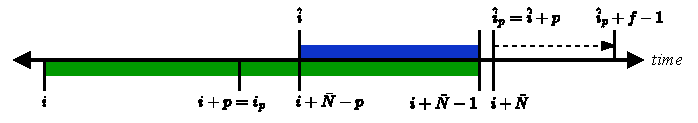
\includegraphics[trim={0.0cm 0.1cm 0.0cm 0.0cm},clip,width=8.4cm]{docs/manuscript/figures/intervals_DeePC.pdf}%[trim={0.0cm 0.0cm 0.0cm 0.0cm},clip,scale=1.0][trim={0.5cm 0.8cm 0.8cm 0.3cm},clip,width=8.4cm]
% 	\caption{Past data from the green ($\datavec{u}{i,\bar{N}},\datavec{y}{i,\bar{N}}$) and blue ($\datavec{u}{\hat{i},p},\datavec{y}{\hat{i},p}$) intervals, shown overlapping as with fully adaptive implementations (for which $i+\bar{N}=\hat{i}_p$), is used to form an output predictor for the black, dashed future prediction window of length $f$. \ac{CL-DeePC} can employ more sample trajectories $N$ of the green window than \ac{DeePC} because its sample trajectories are shorter (due to a shorter prediction window length $f_\mathrm{ID}$ that is used implicitly for identification).}
% 	\label{fig:intervals_DeePC}
% \end{figure}

Without knowledge of the system matrices $\{A,B,C,D,K\}$ and the initial state $x_\mathrm{ini}$, but given sufficiently informative past input-output data from  intervals $k\in[i,\,i+\bar{N})$ and $k\in[\hat{i},\,\hat{i}_p)$ that may overlap\footnote{Depending on the difference $\hat{i}-i>0$ and the number of samples $\bar{N}$.} and have been collected in closed-loop, the principal goal is to find an unbiased behavioural output predictor to replace the unknown relations \eqref{eq:SS_iter} and \eqref{eq:x_ini}.